% !TEX encoding   = UTF8
% !TEX spellcheck = ru_RU
% !TEX root = ../seminars.tex

%%===========================
\chapter{Работа в \name{IDE}}\label{chap:ide}
%%===========================
В~ходе студенческой лабораторной работы по~физике получены данные измерений некоторой величины~\(y\), которая описывается линейной зависимостью \(y = a + bx\), где \(a\)~и \(b\) "--- какие-то константы. Полученные точки записаны в~файл, следуя простому формату:
\[
\begin{array}{ll}
    x_1 & y_1 \\
    x_2 & y_2 \\
    \vdots & \vdots \\
    x_N & y_N \\
\end{array}
\]
Количество пар координат не~указано и может быть произвольным. Несмотря на~линейную зависимость, точки не~ложатся строго на~прямую из-за различного рода погрешностей измерений.

Давайте напишем программу, которая считывает данные эксперимента из~файла и методом наименьших квадратов вычисляет коэффициенты \(a\) и \(b\), а также доверительные интервалы \(\pm\Delta a\) и \(\pm\Delta b\) соответственно.



%%==================================
\section{Метод наименьших квадратов}
%%==================================

%%===============================
\subparagraph{Постановка задачи.}
%%===============================
Рассмотрим регрессию (зависимость) следующего вида:
\begingroup
\newcommand{\SumN}{\ensuremath{\sum\limits_{i=1}^{N}}}
\[
y_i = a + b x_i + \varepsilon_i,\quad i = \overline{1, N}.
\]
Среди всевозможных значений \(\{ a, b \}\) будем искать такие, которые приводят к~минимальной сумме квадратов отклонений (ошибок):
\[
S_{\varepsilon} = \SumN \varepsilon_i^2 = \SumN (y_i - a - b x_i)^2\quad\rightarrow\quad \min\limits_{a, b}.
\]
Запишем условие существования экстремума:
\[
\begin{array}{l}
    \dfrac{\partial}{\partial a} S_{\varepsilon} = -2 \SumN (y_i - a - b x_i) = 0, \\[2ex]
    \dfrac{\partial}{\partial b} S_{\varepsilon} = -2 \SumN (y_i - a - b x_i) x_i = 0, \\
\end{array}
\]
откуда получим систему линейных уравнений:
\[
\left\{ \begin{array}{l}
    \SumN y_i - N a - b\SumN x_i = 0, \\[2ex]
    \SumN x_i y_i - a\SumN x_i - b\SumN x_i^2 = 0. \\
\end{array} \right.
\]
Вводя обозначение для среднего арифметического множества значений некоторой величины \(f\):
\[
\bar f = \dfrac{1}{N}\SumN f_i,
\]
перепишем систему в~виде:
\[
\left\{ \begin{array}{l}
    \bar y - a - b\bar x = 0, \\
    \overline{x y} - a\bar x - b\overline{x^2} = 0, \\
\end{array} \right.
\]
и получим искомое решение:
\[
\boxed{ \begin{array}{l}
        a = \bar y - b\bar x, \\
        b = \dfrac{\overline{x y} - \bar x\bar y}{\overline{x^2} - \bar x^2}. \\
\end{array} }
\]
\endgroup



%%====================================
\subparagraph{Программная реализация.}
%%====================================
Решение этой задачи может быть выражено на~языке \lang{C++} следующим образом:\label{code:lsm}

\cppfile{projects/02/least_squares.cpp}



%%====================
\subparagraph{Сборка.}
%%====================
Чтобы собрать исполняемый файл из командной среды, или <<консоли>>, необходимо перейти в рабочий каталог, где располагается файл с исходным кодом:

\console`$ cd /path/to/your/working/directory`

\noindent и вызвать \GCC:

\console`$ g++  -o lsm  -std=c++17 -pedantic -Wall  least_squares.cpp`


\begin{figure}[h]
{\centering
    \hfill
    \subbottom[точки лежат строго на прямой\label{fig:lsm:a}]{%
        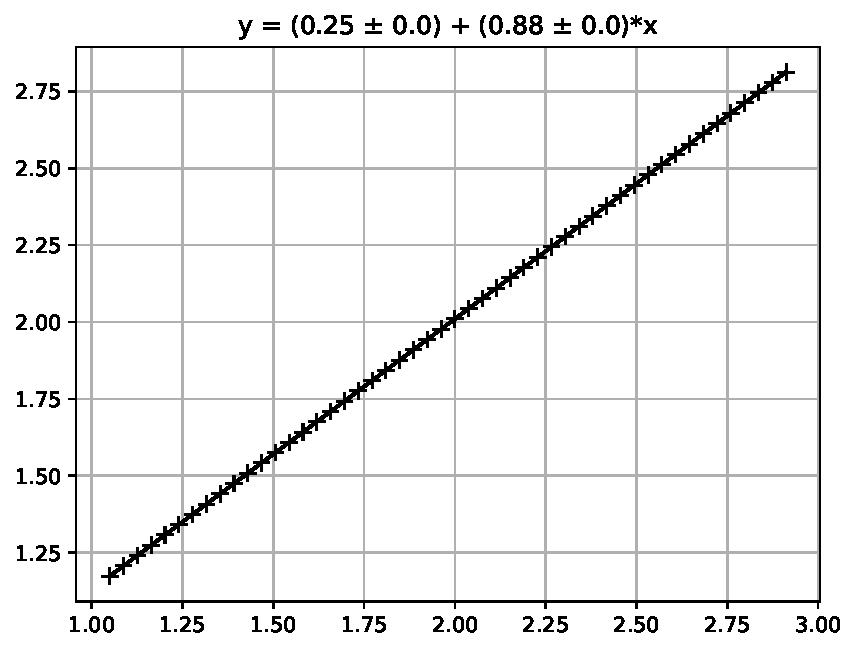
\includegraphics[width=0.45\textwidth]{images/line_exact.pdf}}
    \hfill
    \subbottom[точки не лежат на прямой\label{fig:lsm:b}]{%
        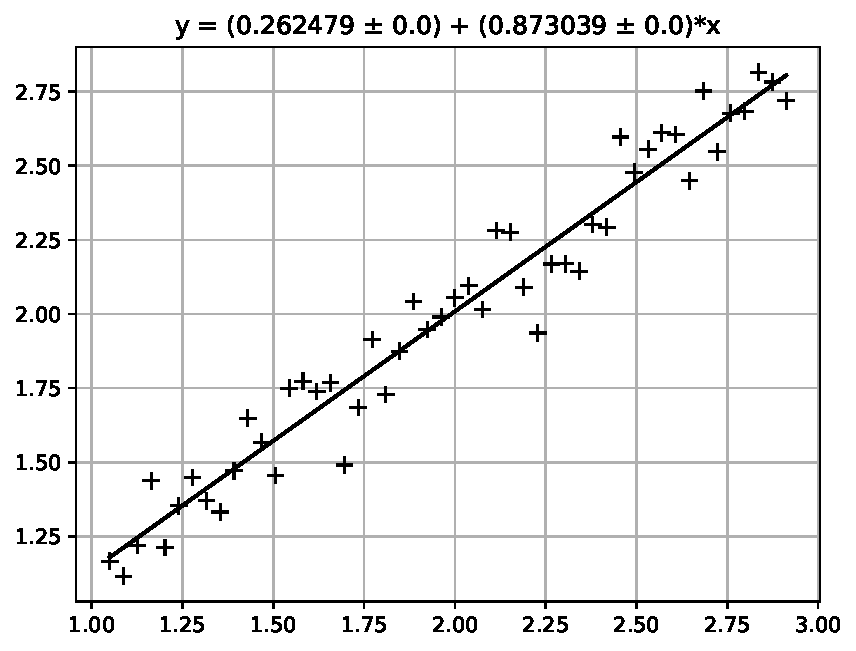
\includegraphics[width=0.45\textwidth]{images/line_approx.pdf}}
    \hfill
}
\caption{Линейная аппроксимация методом наименьших квадратов}
\label{fig:lsm}
\end{figure}



%%==========================
\subparagraph{Тестирование.}\label{test:lsm}
%%==========================
Полученная программа невелика, и, тем не менее, даже она может содержать приличное количество ошибок. Поэтому её работоспособность необходимо как следует проверить, запустив несколько разнообразных тестов. Приведём примеры:
\par\begin{itemfeature}
\item забыли указать имя файла:
\begin{consolecode}
$ ./lsm
usage: ./lsm  file_with_data
\end{consolecode}


\item файл не существует:
\begin{consolecode}
$ ./lsm  not_exist.txt
error: can't open file 'not_exist.txt'
\end{consolecode}


\item файл пуст:
\begin{consolecode}
$ ./lsm  empty.txt
error: division by zero
\end{consolecode}


\item идеальный случай (рис.\,\ref{fig:lsm:a}), когда точки лежат строго на прямой:
\begin{consolecode}
$ ./lsm  line_exact.txt
line_exact.txt  0.25 0  0.88 0
\end{consolecode}


\item реальный случай (рис.\,\ref{fig:lsm:b}), когда точки лежат вдоль прямой с некоторым разбросом:
\begin{consolecode}
$ ./lsm  line_approx.txt
line_approx.txt  0.262479 0  0.873039 0
\end{consolecode}
\end{itemfeature}


\noindent Приведённые данные расположены в архиве
\begin{flushleft}
    \yadisk{cpp-seminars/examples/02.zip}.
\end{flushleft}



%%================
\WhatToReadSection
%%================
\textcite{Stroustrup:2016:ru}: \textbf{глава~4}



%%===============
\ExercisesSection
%%===============
\begin{exercise}
\item Доработайте программу, приведённую на странице~\pageref{code:lsm}. В функции \code{least\_squares} необходимо дополнительно вычислить доверительные интервалы.

Обязательно протестируйте вашу программу. Воспользуйтесь файлами, упомянутыми в подразделе на странице~\pageref{test:lsm}.


\item\hard\label{ex:plot} Продолжая предыдущее упражнение, напишите на \emph{любом} известном вам языке программу, которая рисует график, отражающий результаты лабораторной работы. На вход подаётся исходный файл с точками и оценки коэффициентов линейной регрессии.

Организуйте взаимодействие с программой из предыдущего упражнения так, чтобы можно было автоматически передавать входные данные. На выходе необходимо получить изображение на экране или в файле одного из популярных форматов, например \code{PNG}, с графиком, на котором маркерами нанесены экспериментальные точки, и сплошной линией "--- аппроксимирующая прямая.

Например, рисунок~\ref{fig:lsm} получен в результате выполнения этого упражнения с использованием языка \lang{Python}, пакета \name{Matplotlib} и командной среды (см. страницу~\pageref{sect:pyplot}).
\end{exercise}
